\documentclass[aspectratio=1610]{beamer}

\usetheme{KTH}
\usepackage{graphics}
\usepackage[utf8]{inputenc}
\usepackage{color,soul}

\begin{document}

%%%%%%%%%%%%%%%%%%%%%%%%%%%%%%%%%%%%%%%%%%%%%%%%%%%%%%%%%%%%
\begin{frame}

  \vspace{0.02\textheight}

  \begin{Large}
    Evaluation of Feature Selection Methods for Machine Learning Classification of Breast Cancer
  \end{Large}

  \vspace{0.1\textheight}

  \begin{small}
    \textit{
      Author:\qquad Thony Price \& Niklas Lindqvist\\
      Supervisor:\quad Pawel Herman
    }
  \end{small}
\end{frame}

%%%%%%%%%%%%%%%%%%%%%%%%%%%%%%%%%%%%%%%%%%%%%%%%%%%%%%%%%%%%

\usebackgroundtemplate{\vbox{\null\vspace{3mm}
  \hspace{3mm}\pgfuseimage{kthlogosmall}\par
  \vspace{72mm}\hbox{\hspace{-75mm}\pgfuseimage{kthplatta}}}}

%%%%%%%%%%%%%%%%%%%%%%%%%%%%%%%%%%%%%%%%%%%%%%%%%%%%%%%%%%%%

\begin{frame}
  \frametitle{\hfill Agenda}
  \textbf{Feature selection increases classification accuracy of breast cancer while using an Artificial Neural Network
  }
  \pause

  \begin{itemize}
    \item \textcolor{red}{Why} this was studied\pause
    \item \textcolor{red}{How} results are achieved\pause
    \item \textcolor{red}{What} the results conclude
  \end{itemize}
\end{frame}

% ---------- WHY ----------

\begin{frame}
  \frametitle{\hfill About breast cancer}
  \begin{columns}[T]
    \begin{column}{.5\textwidth}
      \begin{block}{}
        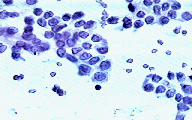
\includegraphics[width=\textwidth]{images/fna_nuclei.png}\\
        Stained tumour cells under microscope
      \end{block}
    \end{column}
    \begin{column}{.5\textwidth}
      \begin{block}{}
        \begin{itemize}
          \item Leading cause of cancer death\pause
          \item Early detection - important!
          \item Detect tumour - then classify\pause
          \item Humans - only 70\% accurate\pause
        \end{itemize}
        \vspace{0.02\textheight}
        \textbf{Solution:} Computer Aided Diagnostics
      \end{block}
    \end{column}
  \end{columns}
\end{frame}

\begin{frame}
  \frametitle{\hfill CAD and Machine Learning}
  \begin{columns}[T]
    \begin{column}{.5\textwidth}
      \begin{block}{}
        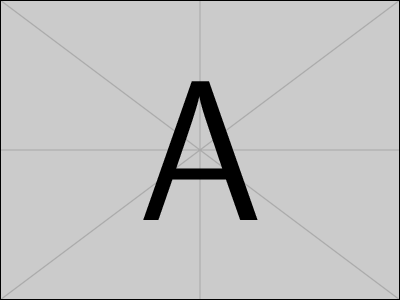
\includegraphics[width=\textwidth]{images/example-image-a.png}\\
        Machine learning concept
      \end{block}
    \end{column}
    \begin{column}{.5\textwidth}
      \begin{block}{}
        \textbf{CAD:} Let the computers do classification to assist radiologist in diagnostics.\pause
        \begin{itemize}
          \item Data with labels\pause
          \item Select model
          \begin{itemize}
            \item Artificial Neural Network
            \item Decision Tree
            \item Na\"ive Bayes'
            \item Support Vector Machine\pause
          \end{itemize}
          \item Train the model\pause
          \item Make predictions\pause
        \end{itemize}
        \vspace{0.02\textheight}
        What \textit{is} the input?
      \end{block}
    \end{column}
  \end{columns}
\end{frame}

% Input with all features
\begin{frame}
  \frametitle{\hfill Input and its features}
  \begin{columns}[T]
    \begin{column}{.5\textwidth}
      \begin{block}{}
        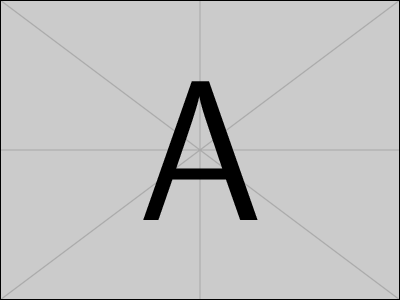
\includegraphics[width=\textwidth]{images/example-image-a.png}\\
        Input image with all features
      \end{block}
    \end{column}
    \begin{column}{.5\textwidth}
      \begin{block}{}
        \begin{itemize}
          \item All features:\\
            $192\times120=23040$
        \end{itemize}
        \vspace{0.02\textheight}
      \end{block}
    \end{column}
  \end{columns}
\end{frame}

% Input with removed features
\begin{frame}
  \frametitle{\hfill Input and its features}
  \begin{columns}[T]
    \begin{column}{.5\textwidth}
      \begin{block}{}
        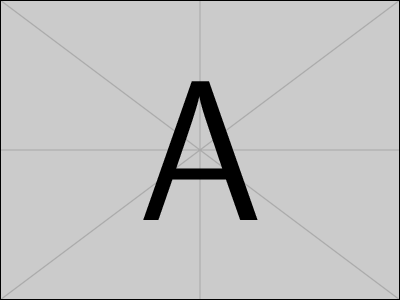
\includegraphics[width=\textwidth]{images/example-image-a.png}\\
        Input image with subset of features
      \end{block}
    \end{column}
    \begin{column}{.5\textwidth}
      \begin{block}{}
        \begin{itemize}
          \item All features:\\
            $192\times120=23040$
          \item Subset of features:\\
            $9000$\pause
          \item How decide what to remove?\\
          \textbf{Feature selection}
        \end{itemize}
        \vspace{0.02\textheight}
      \end{block}
    \end{column}
  \end{columns}
\end{frame}

\begin{frame}
  \frametitle{\hfill Feature selection}
  Two families of feature selection methods was studied\pause
  \begin{columns}[T]
    \begin{column}{.5\textwidth}
      \begin{block}{Filter methods}
        Ranks feature \textit{independently} of ML classifier
      \end{block}
    \end{column}
    \begin{column}{.5\textwidth}
      \begin{block}{Wrapper methods}
        Iteratively evaluates subsets of features in conjunction with ML classifier
      \end{block}
    \end{column}
  \end{columns}
\end{frame}

\begin{frame}
  \frametitle{\hfill So why?}
  To answer:\\
  \vspace{0.05\textheight}
  Can feature selection help improve classification accuracy of breast cancer?\\
  \vspace{0.05\textheight}
  If so, which classification methods can expect such improvement?\\
\end{frame}

% ---------- HOW ----------

\begin{frame}
  \frametitle{\hfill Image summarising the method}
  \begin{figure}[htp]
    \centering
    \makebox[\textwidth]{
    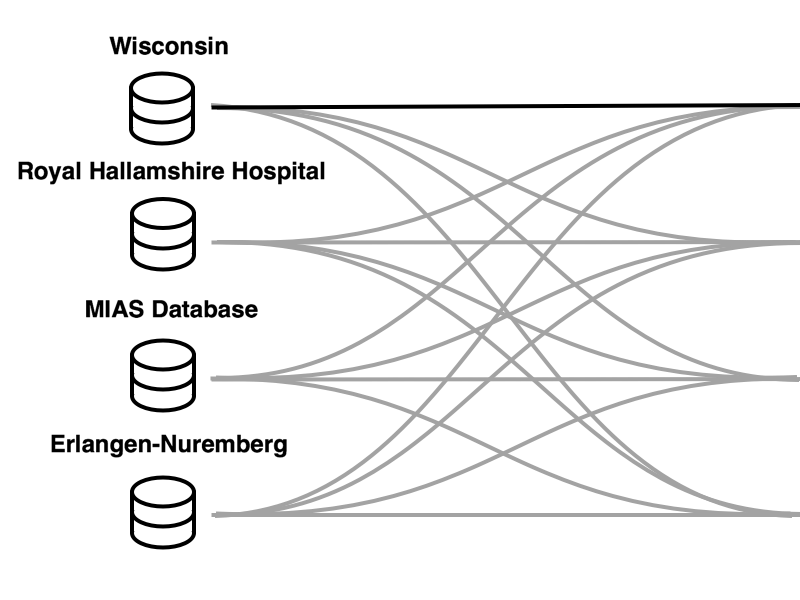
\includegraphics[width=.45\textwidth]{images/KexDbasbild2PNG.png}
    \pause
    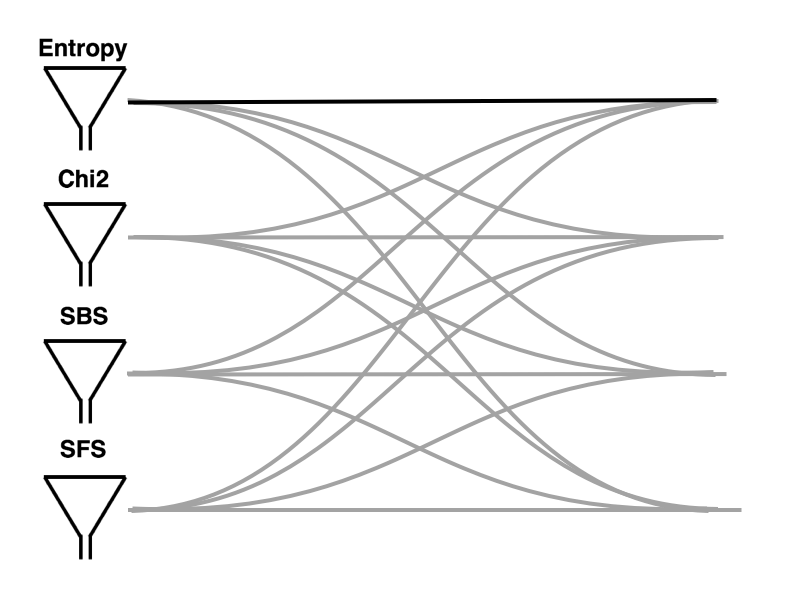
\includegraphics[width=.41\textwidth]{images/KexFilterBildPNG.png}\pause
    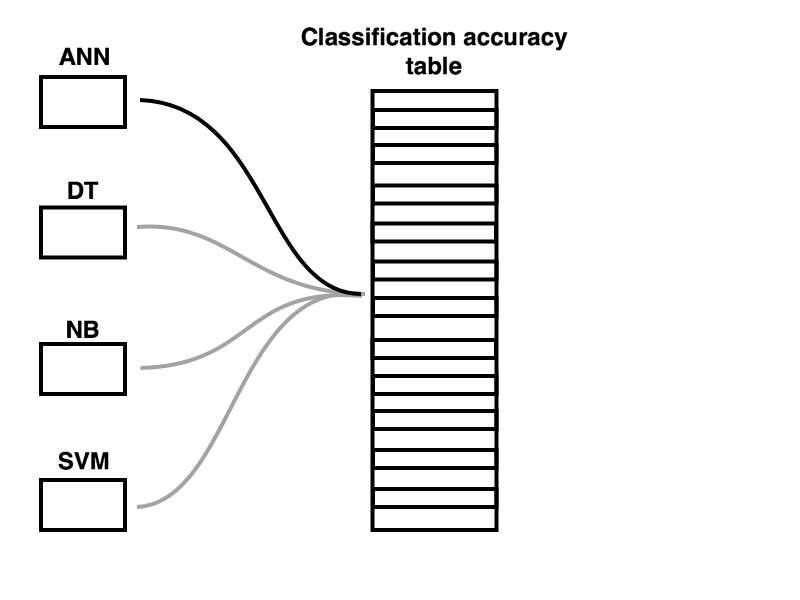
\includegraphics[width=.36\textwidth]{images/kexMLCbildPNG.png}\pause
    }
  \end{figure}
  A total of 800 combinations is calculated
\end{frame}

% ---------- WHAT ----------

\begin{frame}
  \frametitle{\hfill Classification improvements}

    \centering
    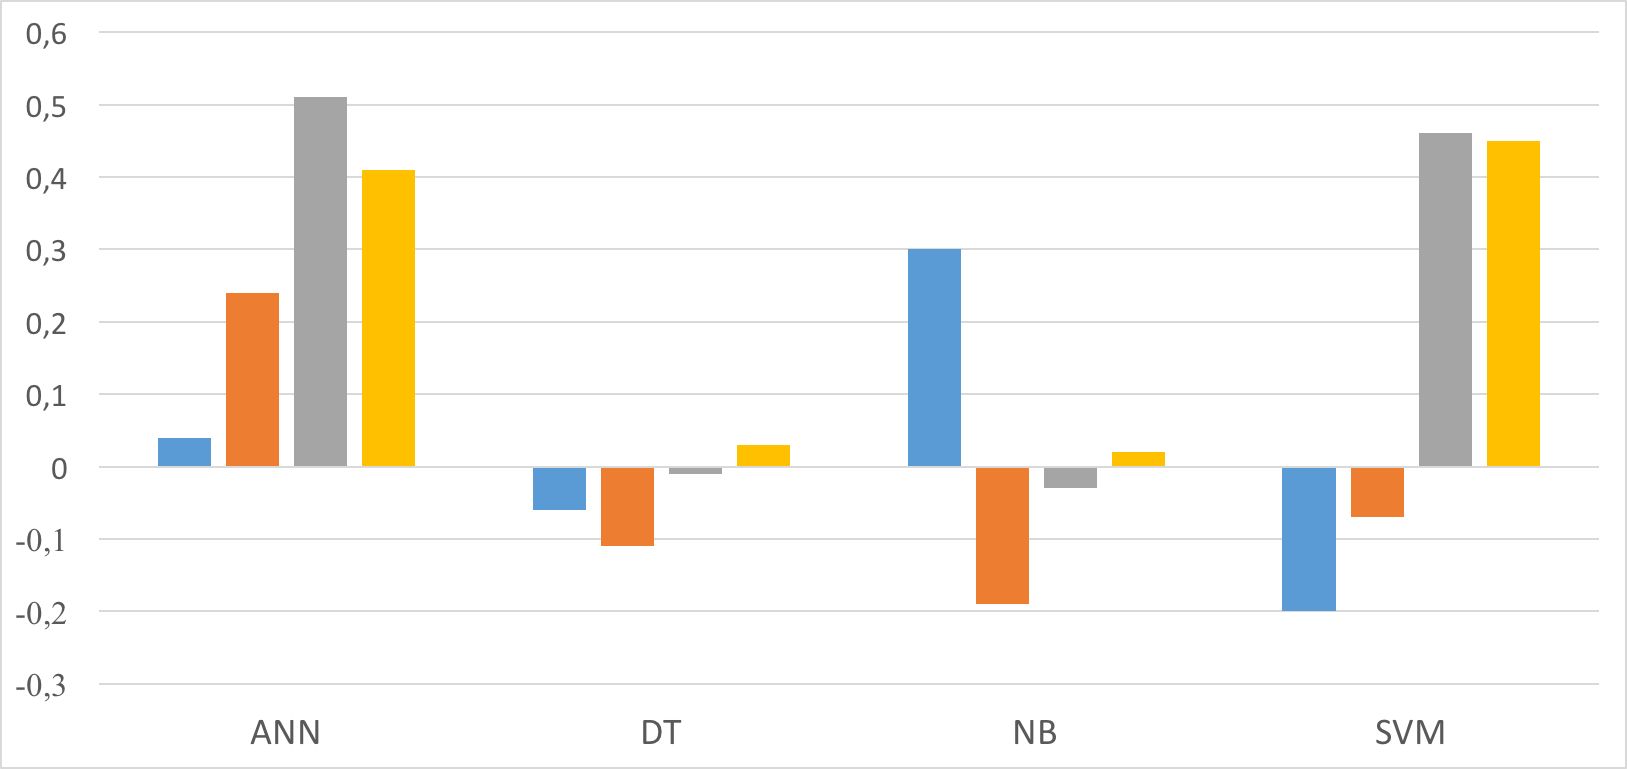
\includegraphics[width=0.9\textwidth]{images/accuracy_improv.png}
    \vspace{0.02\textheight}\\
    t-test shows ANN improvement is significant
\end{frame}

\begin{frame}
  \frametitle{\hfill Proving the improvement - 2 way ANOVA}
  Three factors; Datasets, Feature selection methods, Classifiers.\\
  Which of these affect our results?\pause
  \vspace{0.02\textheight}\\
  \makebox[1.15\textwidth]{
  \begin{columns}[T]
    \begin{column}{.35\textwidth}
      \begin{block}{}
        ANOVA entails interaction between classifiers and feature selection method has a significant effect on accuracy.
        \vspace{0.02\textheight}\\
        Image: Visualising the interaction
      \end{block}
    \end{column}
    \begin{column}{.65\textwidth}
      \begin{block}{}
        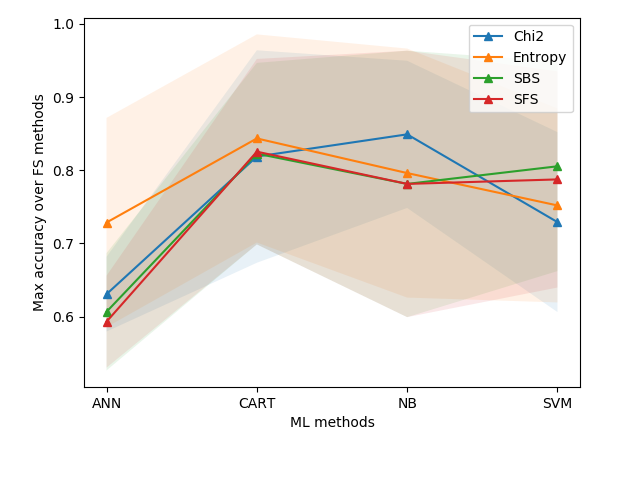
\includegraphics[width=\textwidth]{images/comp_classif_datasets.png}\\
      \end{block}
    \end{column}
  \end{columns}
  }
\end{frame}

\begin{frame}
  \frametitle{\hfill Conclusion}
  \begin{itemize}
  \item Applying feature selection methods to a Artificial Neural Network improved classification accuracy of benign or malignant breast cancer. \\ \pause

  \item RNA data looks promising, over 1900 features \\ \pause

  \item Wrappers or Filter methods? \\ \pause

  \item \textbf{Using all data does not always bring the best results}

    % - No proven increase or decrease of accuracy of Decision Tree, Na\"ive Bayes and Support Vector Machine \pause
  \end{itemize}
\end{frame}

\begin{frame}
  \frametitle{\hfill }
  Thank you for listening
\end{frame}



\begin{frame}
  \frametitle{\hfill Making a KTH Presentation (Example slide)}

  \begin{block}{Steps needed}
    \begin{itemize}
    \item Copy the following files:
    \begin{itemize}
    \item \texttt{examplepresentation.tex} (this file)
    \item \texttt{beamerthemeKTH.sty}
    \item \texttt{kthgraphics} (with all its contents)
    \end{itemize}
    \item Replace the contents in \texttt{examplepresentation.tex} with your own
    \item Run \texttt{pdflatex} a couple of times
    \item Present your slides using a PDF-viewer
    \end{itemize}
  \end{block}

\end{frame}


\end{document}
